\chapter{Methylation based plasmid binning using nanopore sequencing}
\label{chap:mdr}

\textbf{Portions of this chapter originally appeared in:} \\
Fan Y, Bergman Y, Workman R, Simner P, Timp W. Methylation based plasmid binning using nanopore sequencing. Currently unpublished.

\section{Abstract}
\label{sec:abstract}

Genomic analysis of microbial communities often involves reconstructing the full genomic complement of the community members after shotgun sequencing. However, contigs generated by metagenome assemblers typically only represent fragments of genomes and need to be further grouped together, a process known as ‘binning.’ Typical metagenomic binning methods rely primarily on signals from differential coverage and kmer spectra, but these can be confounded by mobile genetic elements, e.g. plasmids, since they can replicate independently of the chromosome and horizontally transfer between organisms. Current methods to resolve mobile genetic elements require more complex sample preparation or matched pairs of sequencing runs, making them more expensive and less accessible. A less used virtue of microbial systems is the “methylation fingerprint” where different bacteria have different methylation signatures as part of their restriction-modification (R-M) system. Using this, we tested the efficacy of metagenomic binning using methylation signal from a single ONT sequencing run. We find that we can correctly bin plasmids in a standard microbial community sample, and that we can identify a single plasmid appearing in different bacterial hosts. Furthermore, we applied this method to a clinical sample, and find that the results are largely consistent with binning methods based on proximity ligation.

\section{Introduction}
\label{sec:intro}

Metagenomics is the analysis of DNA extracted from whole microbial communities for resolving and linking the identities and functions of the community members \citep{Strous2012-nm}. Common analysis steps involve assembling raw sequence reads into contigs, and clustering, or ‘binning’ them into metagenome assembled genomes (MAGs). Ideally, each MAG then represents the complete genetic complement of a community member, including any non-chromosomal DNA. From these MAGs, microbes can then be identified and genomic potential for functions such as metabolism, antimicrobial resistance, and pathogenicity can be inferred.

A number of computational tools have been developed for binning, the vast majority of which rely on k-mer spectra and coverage signals to differentiate between contigs originating from different organisms \citep{Yue2020-cm}. While these methods work well for binning chromosomal contigs, they struggle to effectively bin plasmids \citep{Beaulaurier2018-mu}. This is because plasmids are mobile elements which replicate independently from the bacterial chromosome, characteristics which confound the two key signals most binning methods rely upon.

Molecular biology methods like proximity ligation (Hi-C) have been used to successfully link MGEs and their hosts’ chromosomes \citep{Burton2014-yu}. DNA inside of intact cells is crosslinked, then extracted and fragmented. Crosslinked fragments of DNA are then ligated together, and sequenced on a single read. Reads partially aligning to a chromosome and partially aligning to an MGE then provides evidence that the chromosome and MGE originated in a single cell. While this method has been shown to work well, it’s still somewhat limited by its need for two sequencing runs, intact bacterial samples, and longer, more labor intensive library preparation \citep{Beyi2021-tv}.

More recently, binning methods that use DNA methylation detected by single molecule sequencing technologies have emerged \citep{Beaulaurier2018-mu, Tourancheau2021-hv}. These methods take advantage of the restriction-methylation systems in bacteria, which cause unique strains of bacteria to exhibit DNA methylation at potentially unique combinations of motifs. Importantly, these methylation patterns remain consistent across all of the chromosomes and plasmids of an individual strain, making them useful for associating any non-contiguous segments of DNA to each other. Methylation based binning with the Pacific Biosciences (Pacbio) single molecule real time (SMRT) sequencing platform relies on detecting pauses in the raw fluorescence signal (interpulse duration; IPD) to detect methylation. Currently available methods using the Oxford Nanopore Technologies (ONT) platform rely on comparing the raw electrical data generated by ONT sequencers in matched runs of methylated native DNA and completely unmethylated whole genome amplified (WGA) DNA \citep{Tourancheau2021-hv}. Characteristic differences in electrical signal between the two runs can be used to locate and identify methylation. While this also works well, it requires two ONT sequencing runs and additional preparation work (WGA), again increasing the cost and limiting the scope of the method.

Here, we demonstrate a framework to perform metagenomic binning using methylation calls from a single single molecule sequencing run. Recent modifications to the BAM file specification have enabled base modification calls to be encoded from either PacBio or ONT data directly in the BAM file.  In our case, we used Megalodon to call methylation, a tool part of ONT’s stack of software, in conjunction with the all-context 5mC and 6mA modification model in Rerio, ONT’s suite of ‘research release’ basecalling models. On each metagenomic contig or reference sequence, we determine the methylation level at a combination of motifs, and use similarities in methylation levels at these motifs for binning. To assess binning performance, we examine a shared plasmid in a two-bacteria system, as well as a simple, synthetic microbial community. We then extend the method to a human microbiome sample, and compare to Hi-C results on the same sample.


\section{Results and Discussion}
\label{sec:results}

\subsection{Microbial Community Standard}
\label{sec:zymo}

To test the feasibility of associating plasmids to chromosomes, we used the ZymoBIOMICS Microbial Community Standard, which contains seven different species of bacteria and one yeast {\bf Table \ref{tab:motifsummary}}. Among the bacteria in this sample, the E. coli strain contains a 110kb plasmid, and the S. aureus strain contains 3 plasmids with lengths 6.3kb, 2.2kb, and 2.9kb. As the identity of each species in the sample is known, we used their reference genomes to call methylation, and use these methylation signatures to bin plasmids with bacterial chromosomes.




\begin{table}[!hb]
\centering
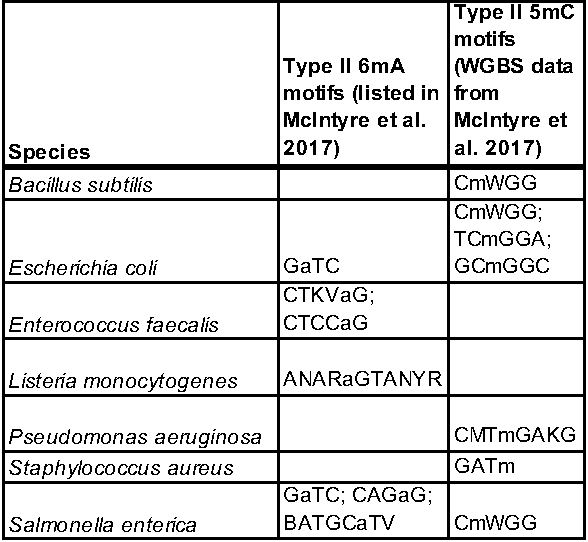
\includegraphics[width = .5\linewidth,keepaspectratio]{figure/motifsummary.pdf}
\caption[Summary of known methylation motifs in the ZymoBIOMICS sample.]{{\bf Summary of known methylation motifs in the ZymoBIOMICS sample..} 5mC modifications are denoted as 'm,' and tmA motifs are denoted as 'a.' }
\label{tab:motifsummary}
\end{table}



To select the ‘barcode,’ or set of methylation motifs that would best differentiate between the species in the sample, we used the 6mA motifs and WGBS data published in McIntyre \citep{McIntyre2017-ed} et al. From the WGBS data, we identified the short (<8bp) 5mC motifs methylated in each species, and confirmed that these short motifs account for >99\% of all 5mC methylation in these species {\bf Table \ref{tab:bisulf}}. For both 6mA and 5mC motifs, only the short motifs of Type II and Type III MTases were included, since they comprise 85 of the 100 most frequently occurring methylation specificities listed in REBASE \citep{Roberts2003-ss}. While excluding Type I motifs excludes the potential discriminatory power they provide, it also simplifies analysis by avoiding the long, ambiguous sections of the Type I bipartite motifs, e.g. EcoKI (AAC[N6]GTGC or GCAC[N6]GTT). Due to the absence of many motifs in the short S. aureus plasmids, we further narrowed the barcode to just GATC, CAGAG, CCWGG and CTKVAG {\bf Table \ref{tab:motifsummary}}. Despite this motif reduction, the two shortest S. aureus plasmids still did not have methylation calls for all four motifs {\bf Table \ref{tab:meancov}, Figure \ref{fig:covhists}}, and were therefore excluded from further analysis. According to the WGBS and PacBio data \citep{McIntyre2017-ed} {\bf Tables \ref{tab:motifsummary}, \ref{tab:motifsummary}}, this four-motif barcode is theoretically sufficient to distinguish between all species except L. monocytogenes and P. aeruginosa, neither of which is methylated at any of the four motifs in the barcode. However, this reduction sufficiently preserves the methylation motifs specific to S. aureus and E. coli such that they are uniquely distinguishable from the other species in the sample, enabling us to correctly assign these plasmids to their hosts.


\begin{table}[!hb]
\centering
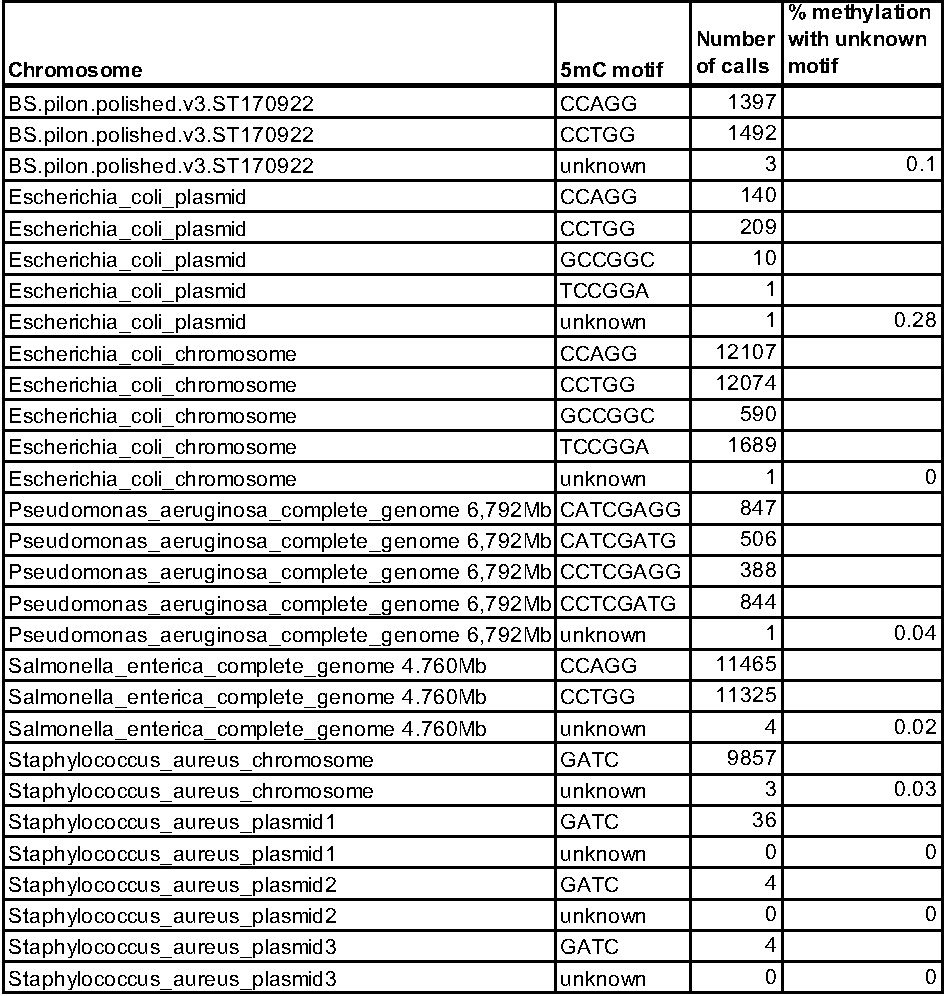
\includegraphics[width = 1\linewidth,keepaspectratio]{figure/bisulf.pdf}
\caption[5mC methylation motifs in the ZymoBIOMICS sample.]{{\bf 5mC methylation motifs in the ZymoBIOMICS sample..} For each DNA sequence in the Zymo sample, counts of 5mC motifs are listed, along with the number of methylation loci not attributable to any of the listed motifs. }
\label{tab:bisulf}
\end{table}


\begin{table}[!hb]
\centering
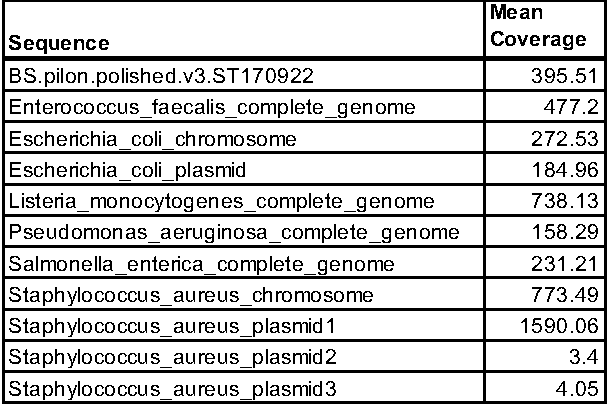
\includegraphics[width = .5\linewidth,keepaspectratio]{figure/meancov.pdf}
\caption[Zymo mean coverage.]{{\bf Zymo mean coverage..} Mean coverage per sequence in the ZymoBIOMICS sample. }
\label{tab:meancov}
\end{table}


\begin{figure}[!hb]
\centering
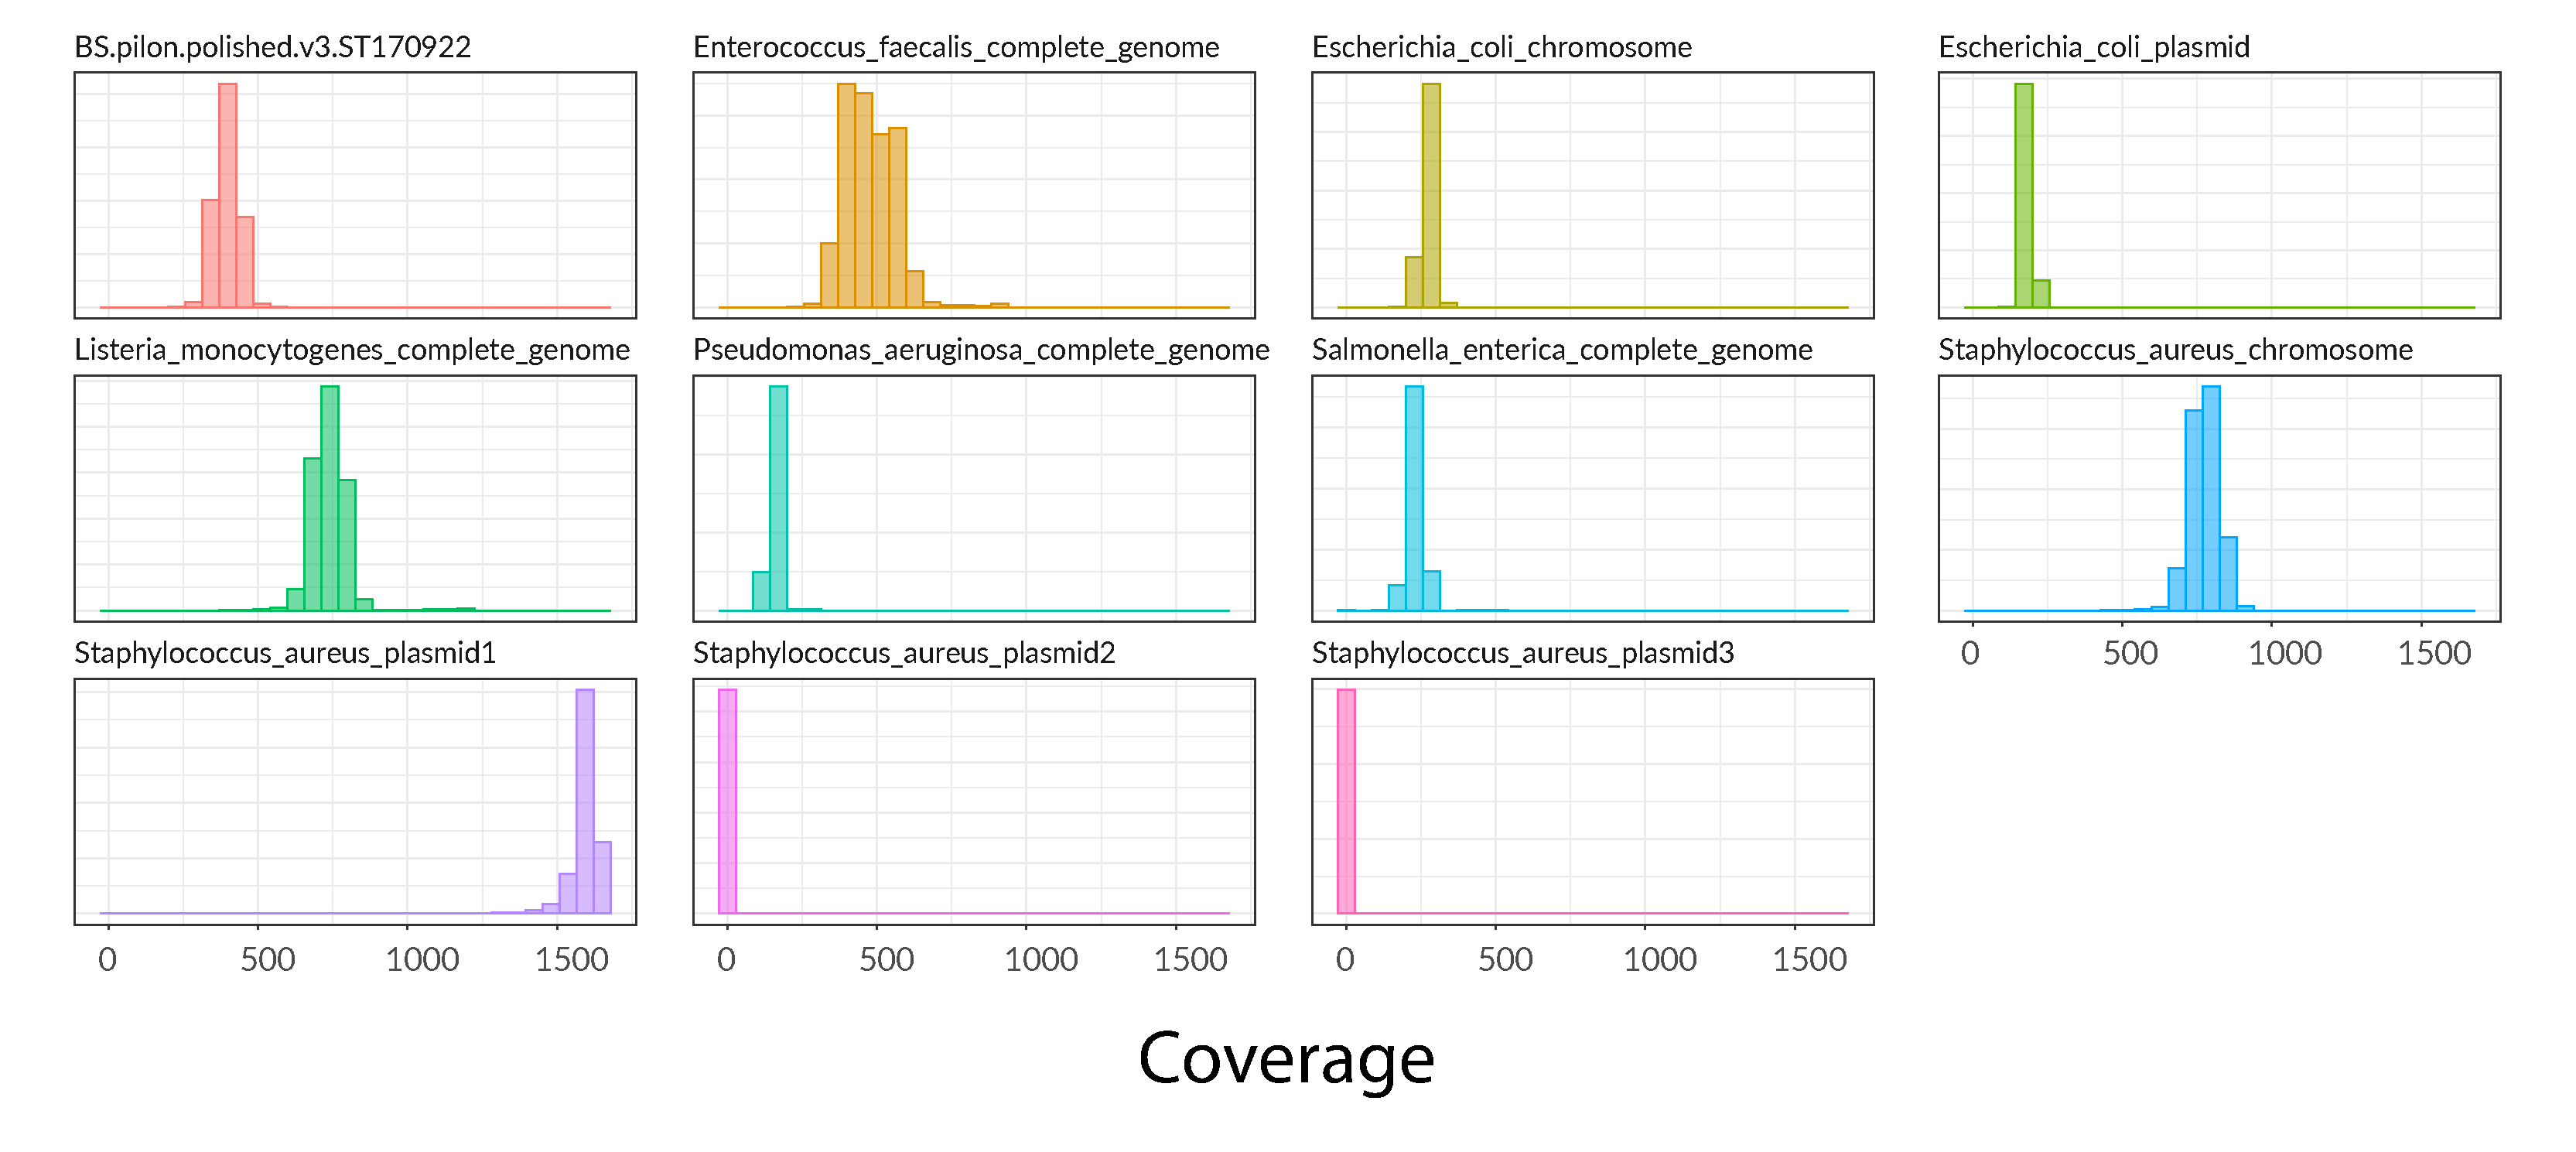
\includegraphics[width = 1\linewidth,keepaspectratio]{figure/covhists.pdf}
\caption[Zymo mean coverage.]{{\bf Zymo mean coverage..} Coverage distributions per sequence in the ZymoBIOMICS sample. }
\label{fig:covhists}
\end{figure}


For each chromosome and plasmid, we constructed a methylation signature consisting of the average percent methylation at each of the four motifs in the barcode {\bf Figure \ref{fig:controls}a}. The percent methylation at each locus is calculated as the number of methylated calls out of the total number of calls made. Euclidean distance between these signatures was then used as a measure of similarity {\bf Figure \ref{fig:controls}b}. Notably, the methylation signatures closest to each of the plasmids correspond to the bacterial chromosomes of the species harboring each plasmid respectively. As expected, the distance between L. monocytogenes and P. aeruginosa are among the smallest between chromosomes because no motif included in the barcode differentiates between them. However, E. faecalis also groups closely with L. monocytogenes and P. aeruginosa. The only motif included in the barcode which separates E. faecalis from L. monocytogenes and P. aeruginosa is a 6mA motif (CTKV6mAG), and upon examination of the methylation signatures themselves, it becomes clear that this motif does not offer as much discriminatory power as the others {\bf Figure \ref{fig:controls}a}. In fact, removing this motif from the barcode does not appreciably change the distances between the chromosomes {\bf Figure \ref{fig:zheatmaps}a}.

\begin{figure}[!hb]
\centering
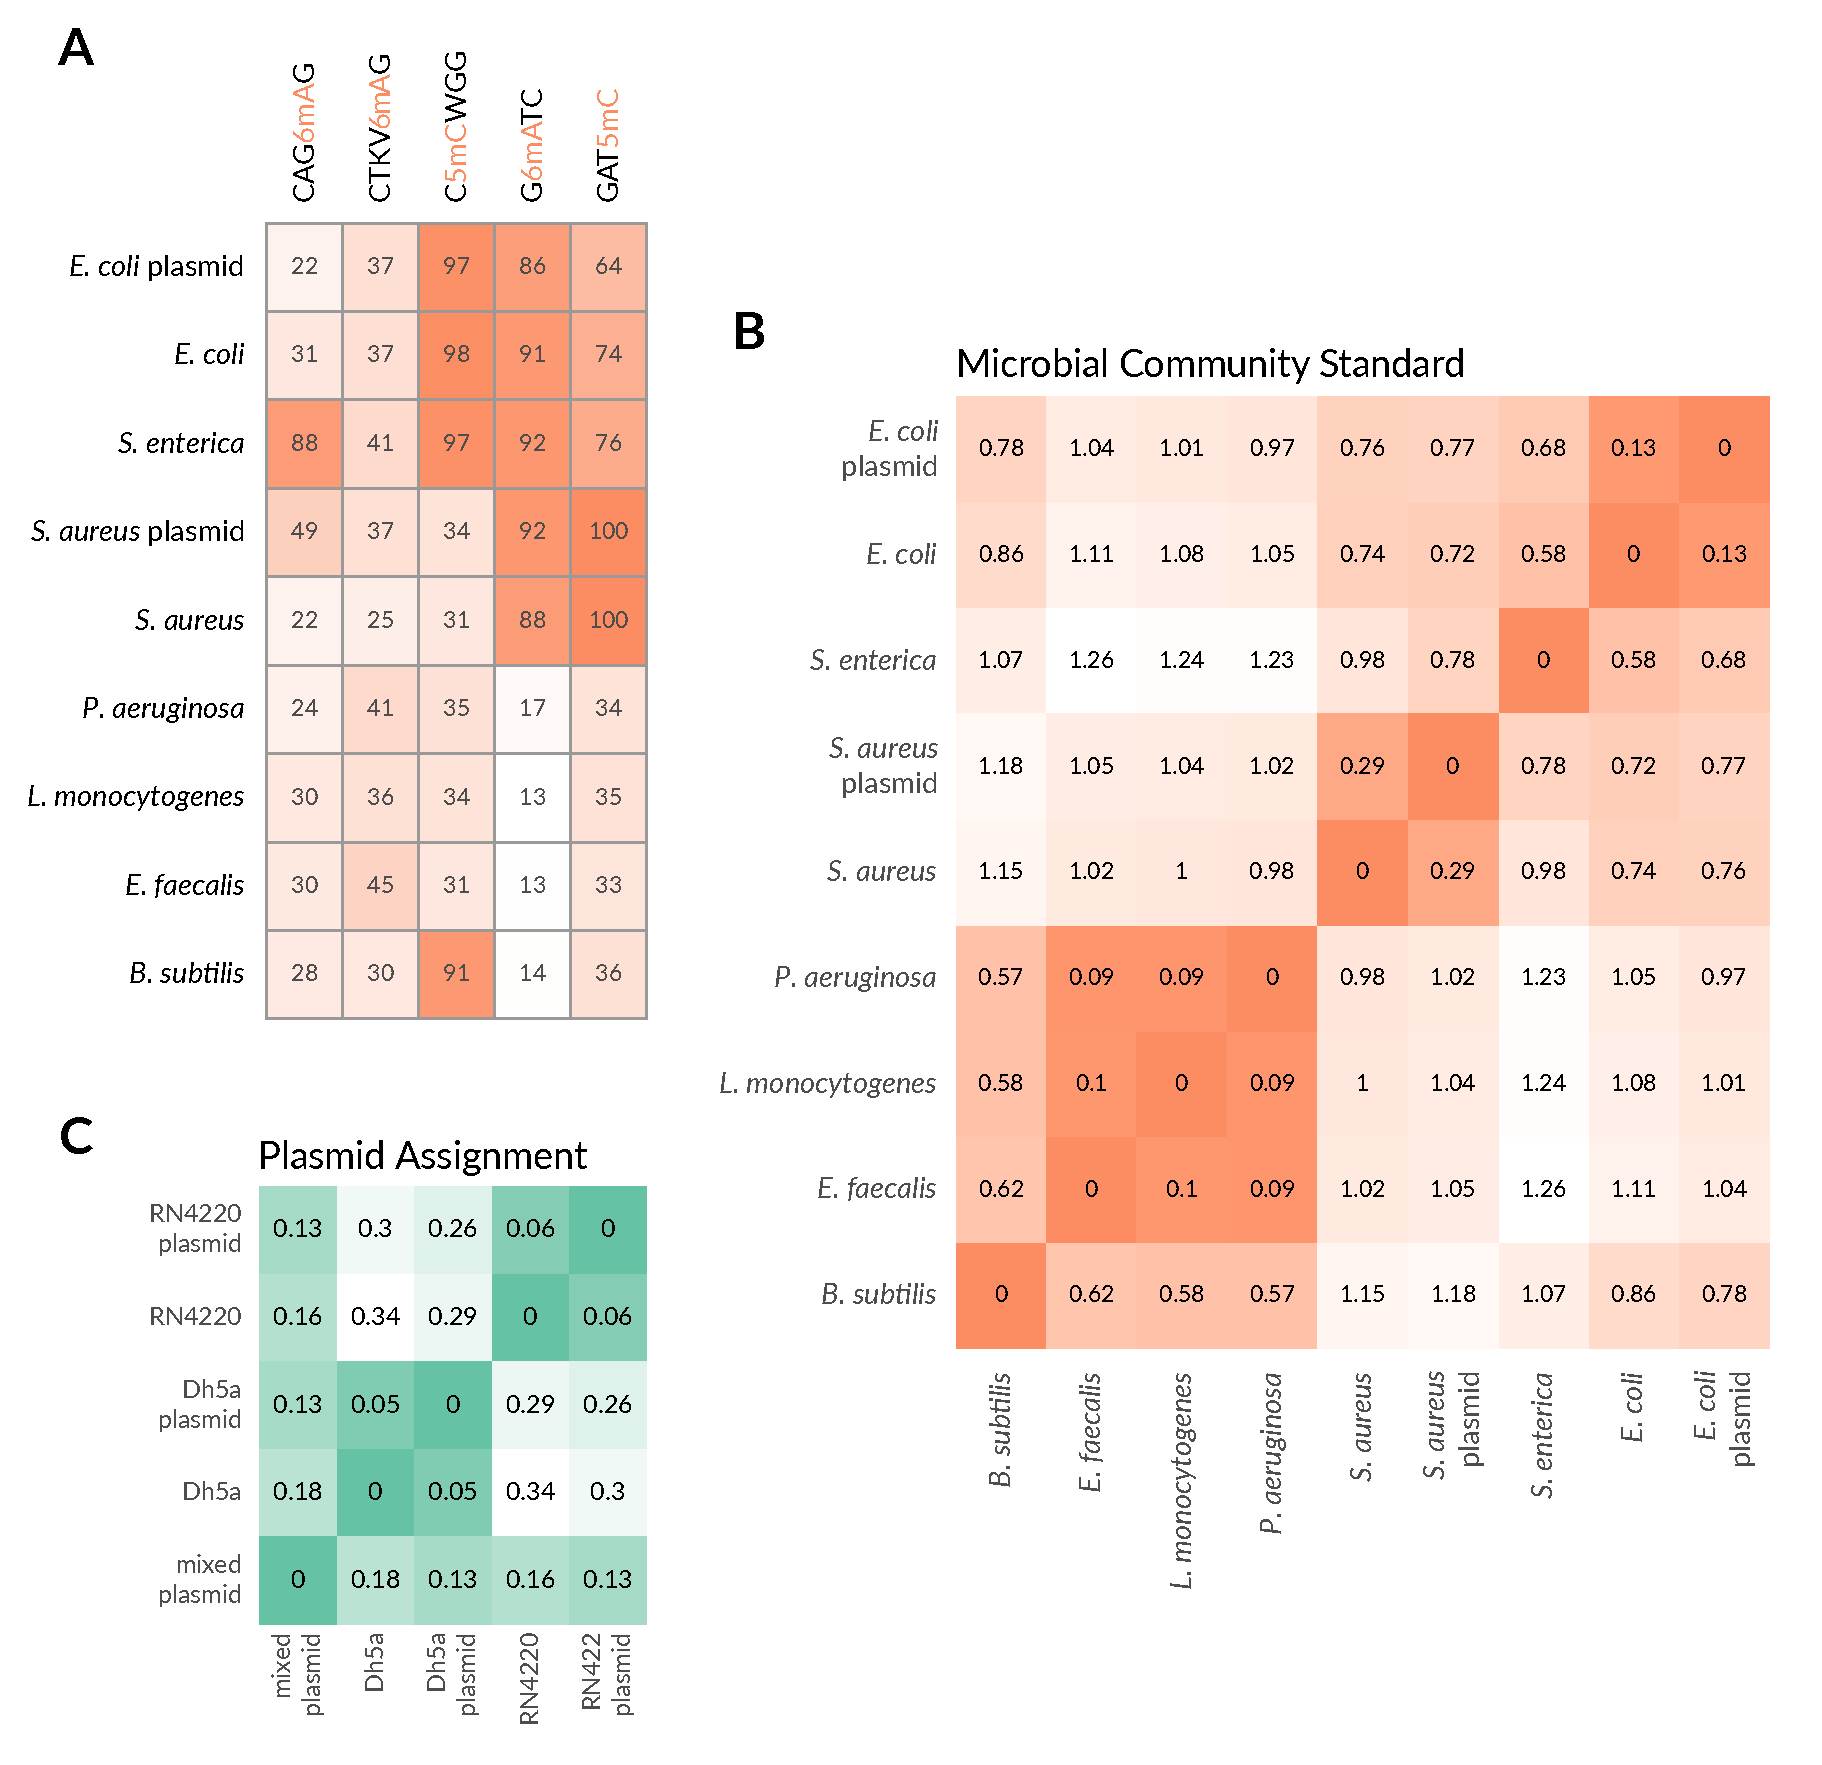
\includegraphics[width = 1\linewidth,keepaspectratio]{figure/controls.pdf}
\caption[Methylation binning in synthetic communities.]{{\bf Methylation binning in synthetic communities..} {\bf (A)} Percent methylation at each motif for each sequence in the Zymo community. {\bf (B)} Methylation distance between sequences in the Zymo community based on the motifs in {\bf (A)}. {\bf (C)} Methylation distance between RN4220, Dh5a, their associated plasmids, and the synthetic mixture of their plasmids, when percent methylation is calculated using normalized coverage. }
\label{fig:controls}
\end{figure}



\begin{figure}[!hb]
\centering
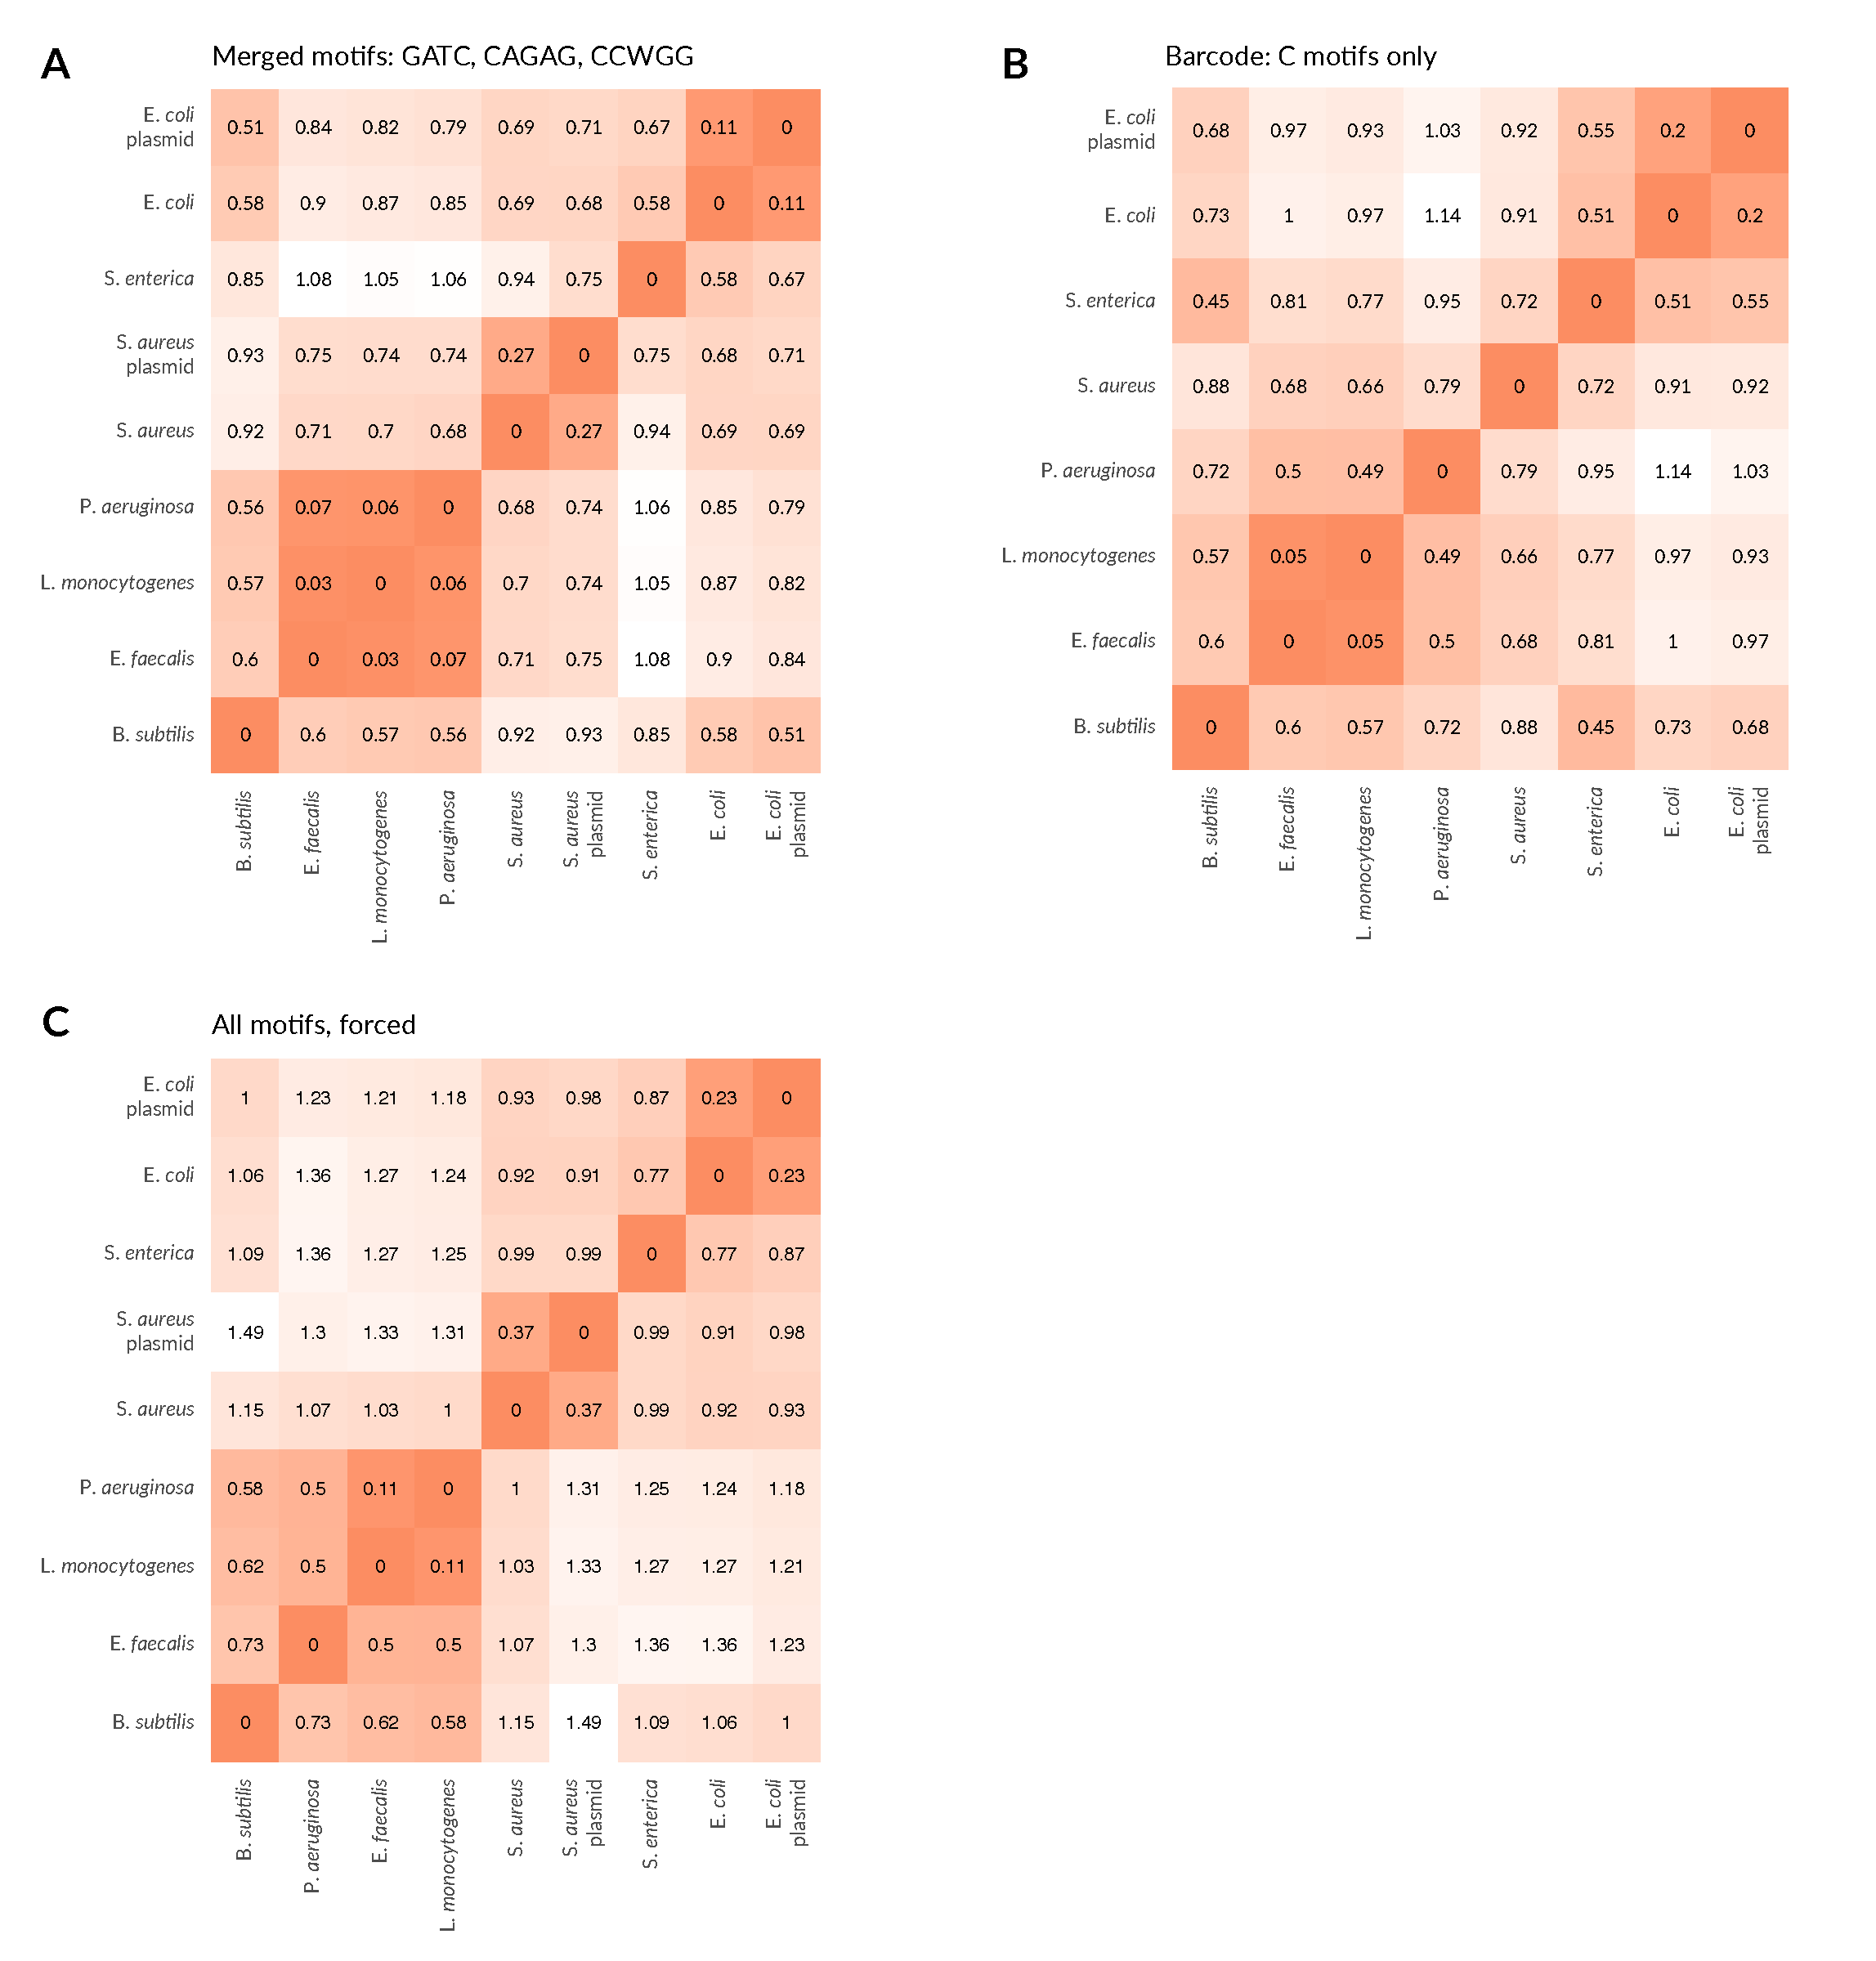
\includegraphics[width = 1\linewidth,keepaspectratio]{figure/zheatmaps.pdf}
\caption[Methylation binning in Zymo community.]{{\bf Methylation binning in Zymo community..} {\bf (A)} Methylation distance between sequences in the Zymo community, based on the motifs GATC, CAGAG, CCWGG where GATC represents both G6mATC and GAT5mC. {\bf (B)} Methylation distance between sequences in the Zymo community, based on only 5mC motifs GATC, CCWGG, GCCGGC, CMTCGAKG. }
\label{fig:zheatmaps}
\end{figure}


To further explore, we implemented a barcode composed of only the relevant 5mC motifs {\bf Table \ref{tab:motifsummary}}. Due to the lack of CMT(5mC)GAKG occurrences on the S. aureus plasmid, we only classified the E. coli plasmid using this all-5mC barcode {\bf Figure \ref{fig:zheatmaps}b}. However, because the newly included CMT5mCGAKG is unique to P. aeruginosa, it is differentiable from L. monocytogenes and E. faecalis using this barcode. As expected, since the L. monocytogenes and E. faecalis strains in this sample do not exhibit any Type II 5mC methylation, these chromosomes remain close together in methylation space.

Methylation distance also can be calculated with tolerance for missing methylation values, where distances with missing values are scaled to as to be comparable to complete distances. By including all 5mC motifs in the barcode and forcing the classification of the S. aureus plasmid, P. aeruginosa again becomes differentiable from L. monocytogenes and E. faecalis {\bf Figure \ref{fig:zheatmaps}c}. However, the distance between the S. aureus plasmid and chromosome also increases. While the shortest distances observed are still attributable to sequences with identical methylation, these distances are not as tight.

Notably, the methylation distances between the species in this community standard do not closely reflect their taxonomic lineages {\bf Figure \ref{fig:taxonomy}}. This indicates that methylome diversity is not determined by phylogeny, and suggests that methylation can potentially be used to distinguish between even closely related organisms.

\begin{figure}[!hb]
\centering
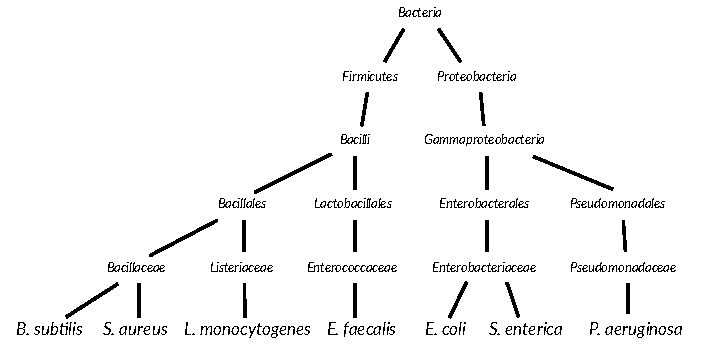
\includegraphics[width = 1\linewidth,keepaspectratio]{figure/taxonomy.pdf}
\caption[Zymo taxonomy.]{{\bf Zymo taxonomy..} Simplified taxonomic lineages of the Zymo microbial community bacteria. }
\label{fig:taxonomy}
\end{figure}


\subsection{Two-bacteria System}
\label{sec:byard}

We then tested the efficacy of methylation signatures for accurately linking a single plasmid to different bacterial hosts. To do this, we used two bacteria, E. coli (strain DH5α) and S. aureus (strain RN4220), each containing an identical 10kb plasmid (pRW62). This plasmid contains an origin of replication for E. coli and a separate origin of replication for S. aureus so that it is replicated in both species. Both were cultured separately and sequenced separately on individual Flongle runs {\bf Figure \ref{tab:yields}}. With bisulfite sequencing data, we observed only two methylated loci in the entire genome of this strain of S. aureus, neither of which are in a known 5mC methylation context. In this strain of E. coli, all 5mC methylated loci occur in a C5mCWGG context.


\begin{table}[!hb]
\centering
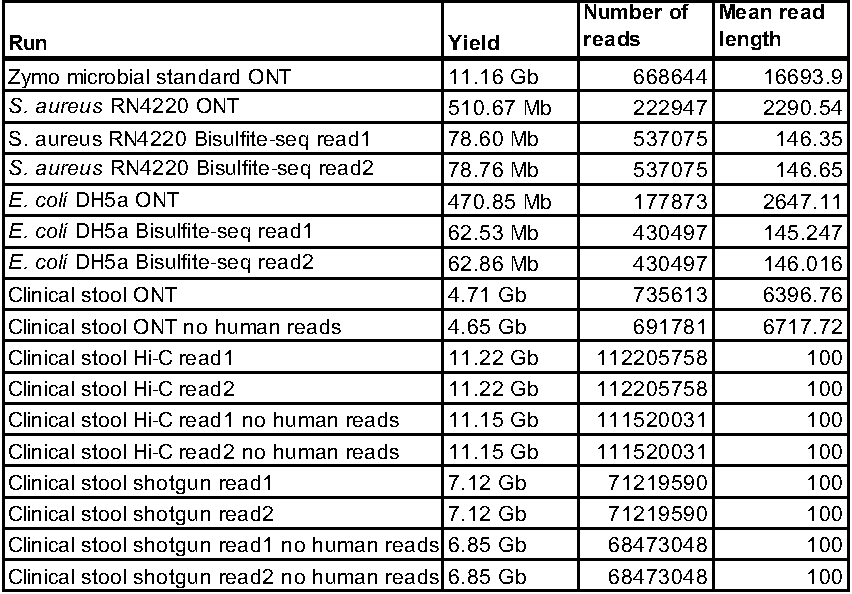
\includegraphics[width = 1\linewidth,keepaspectratio]{figure/yields.pdf}
\caption[ Summary statistics of sequencing runs.]{{\bf  Summary statistics of sequencing runs..} Yield, number of reads, and mean read length for each sequencing run performed. }
\label{tab:yields}
\end{table}


Given the results of bisulfite analysis, we selected frequently recorded motifs in REBASE which include an adenine, as well as CCWGG. This resulted in a barcode of GATC, GANTC, CCWGG, CAGAG, CTKVAG, and GTWWAC. Because the methylated residues are not necessarily known for each motif, the base with the highest methylation percentage was chosen to represent each motif  locus. Again, the methylation signature of each sequence is represented by the average methylation percentages across all loci for each motif.

\begin{figure}[!hb]
\centering
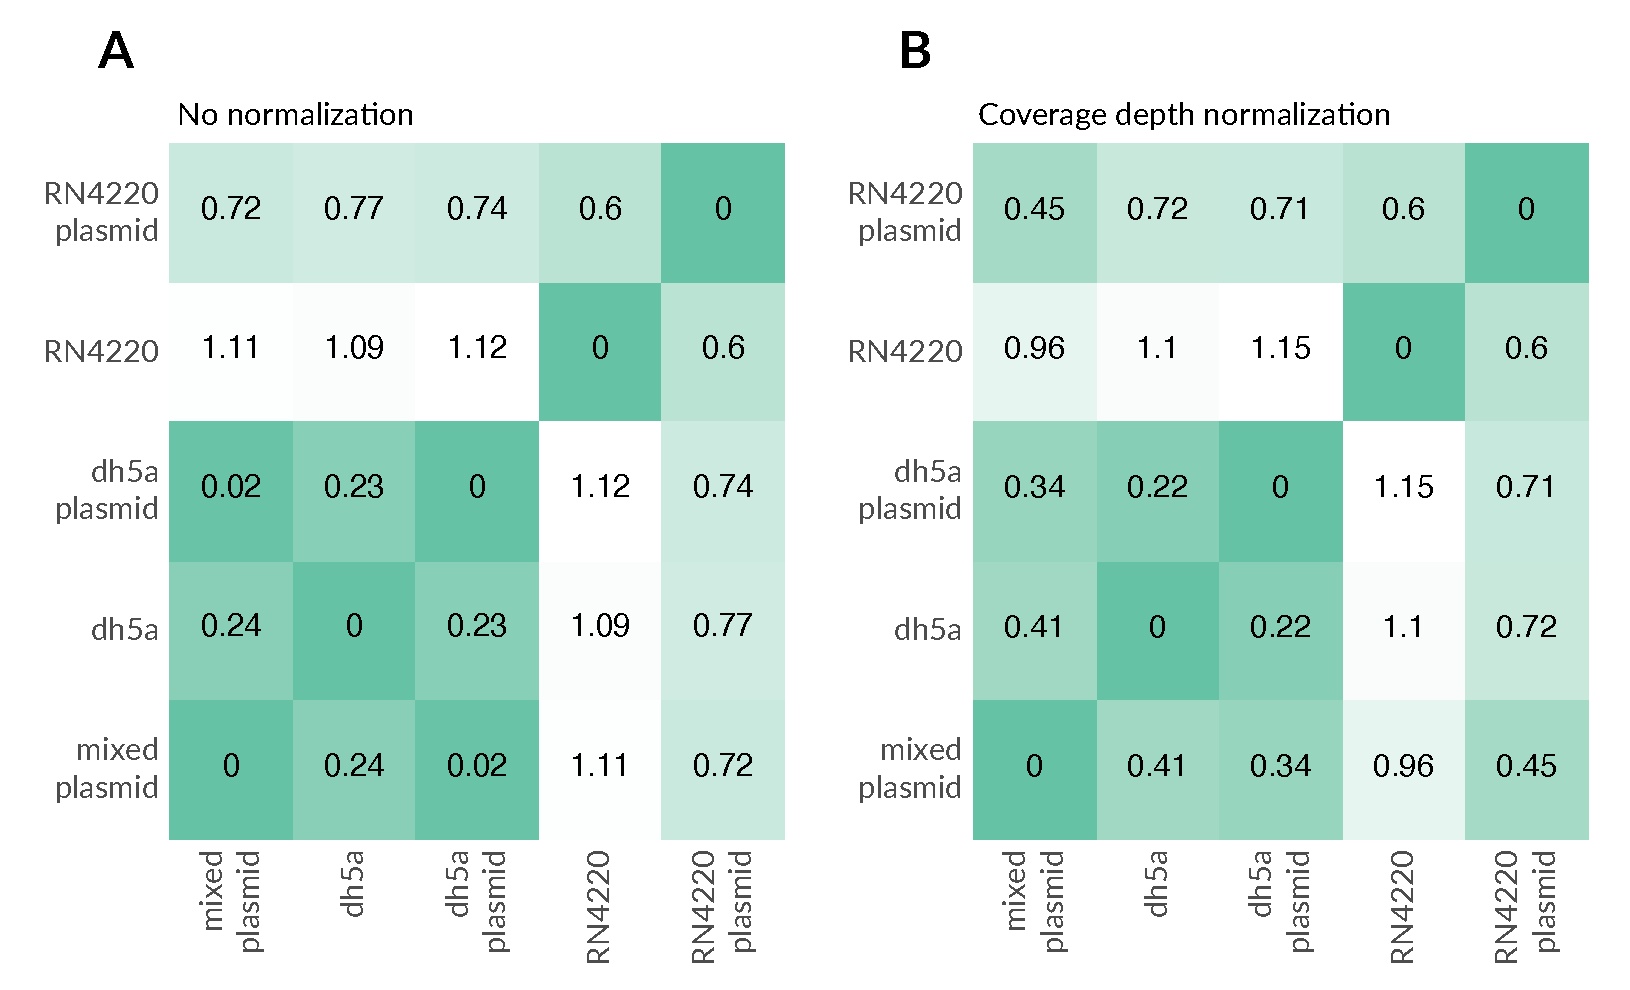
\includegraphics[width = 1\linewidth,keepaspectratio]{figure/bheatmaps.pdf}
\caption[Methylation distance between RN4220 and Dh5a.]{{\bf Methylation distance between RN4220 and Dh5a..} {\bf (A)} Methylation distance between RN4220 and Dh5a and plasmids with no normalization. The mixed plasmid comprises all plasmid reads. {\bf (A)} Methylation distance between RN4220 and Dh5a where reads have been randomly downsample such that chromosomes have the same average coverage and individual plasmids have the same average coverage. The mixed plasmid contains the downsampled plasmid reads of both strains. }
\label{fig:bheatmaps}
\end{figure}


Using methylation signatures defined by these five motifs, we are able to distinguish the plasmid’s presence in E. coli from its presence in S. aureus {\bf Figure \ref{fig:controls}c}. However, when plasmid reads from both runs are mixed, combined and analyzed , the methylation signature places the mixed plasmid much closer to the E. coli signature than the S. aureus signature {\bf Figure \ref{fig:bheatmaps}a}. This is partially because this plasmid has a much higher copy number in the E. coli data {\bf Figure \ref{tab:runcov}}. When the E. coli plasmid reads are downsampled from 6000X coverage to 440X coverage to match the sequence coverage of the S. aureus reads before in silico mixing, the mixed plasmid moves away from the E. coli signature {\bf Figure \ref{fig:bheatmaps}b}. Much of the remaining bias is accounted for by the high uncertainty of methylation calls at unmethylated loci {\bf Figure \ref{fig:modprobsfig}}. Methylation callers such as Megalodon or nanopolish compute a probability that a base of a sequencing read is methylated \citep{Simpson2017-wb}. This probability is then thresholded to call bases as either methylated, unmethylated, or uncertain. Though 5-methylcytosine in a CG context gives robust calls of either methylated or unmethylated \citep{Simpson2017-wb}, non-CG 5-methylcytosine models are less robust and 6-methyladenine gives a smaller electrical signal shift, leading to more uncertain calls. Methylated motifs still present a high probability of methylation, but unmethylated motifs are less clear {\bf Figure \ref{fig:modprobsfig}, Table \ref{tab:modprobs}}. Unmethylated loci are less likely to contribute any methylation calls, suggesting that most calls made on the mixed plasmid originated from the E. coli data, the only organism with any confirmed methylation. To counteract this, we calculated methylation percentage as the ratio of methylated calls to the total coverage, instead of total methylation calls, at each locus. This way, the unmethylated calls do not play a role in determining the methylation signatures. With this adjustment, the mixed plasmid falls roughly equidistant between the E. coli and S. aureus signatures {\bf Figure \ref{fig:controls}c}. As methylation callers improve, we expect that this correction may not be necessary, because the values from methylation vs coverage and methylation vs called will converge.

\begin{table}[!hb]
\centering
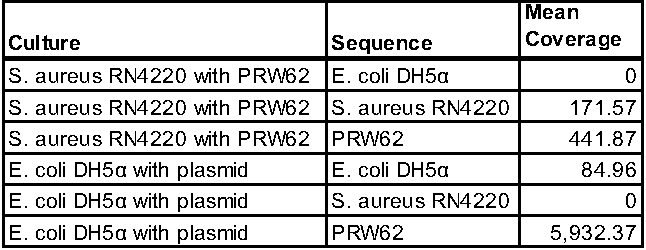
\includegraphics[width = .5\linewidth,keepaspectratio]{figure/runcov.pdf}
\caption[Two-bacteria system coverage]{{\bf Two-bacteria system coverage.} Mean coverage per sequence for each of the two sequenced cultures. }
\label{tab:runcov}
\end{table}



\begin{figure}[!hb]
\centering
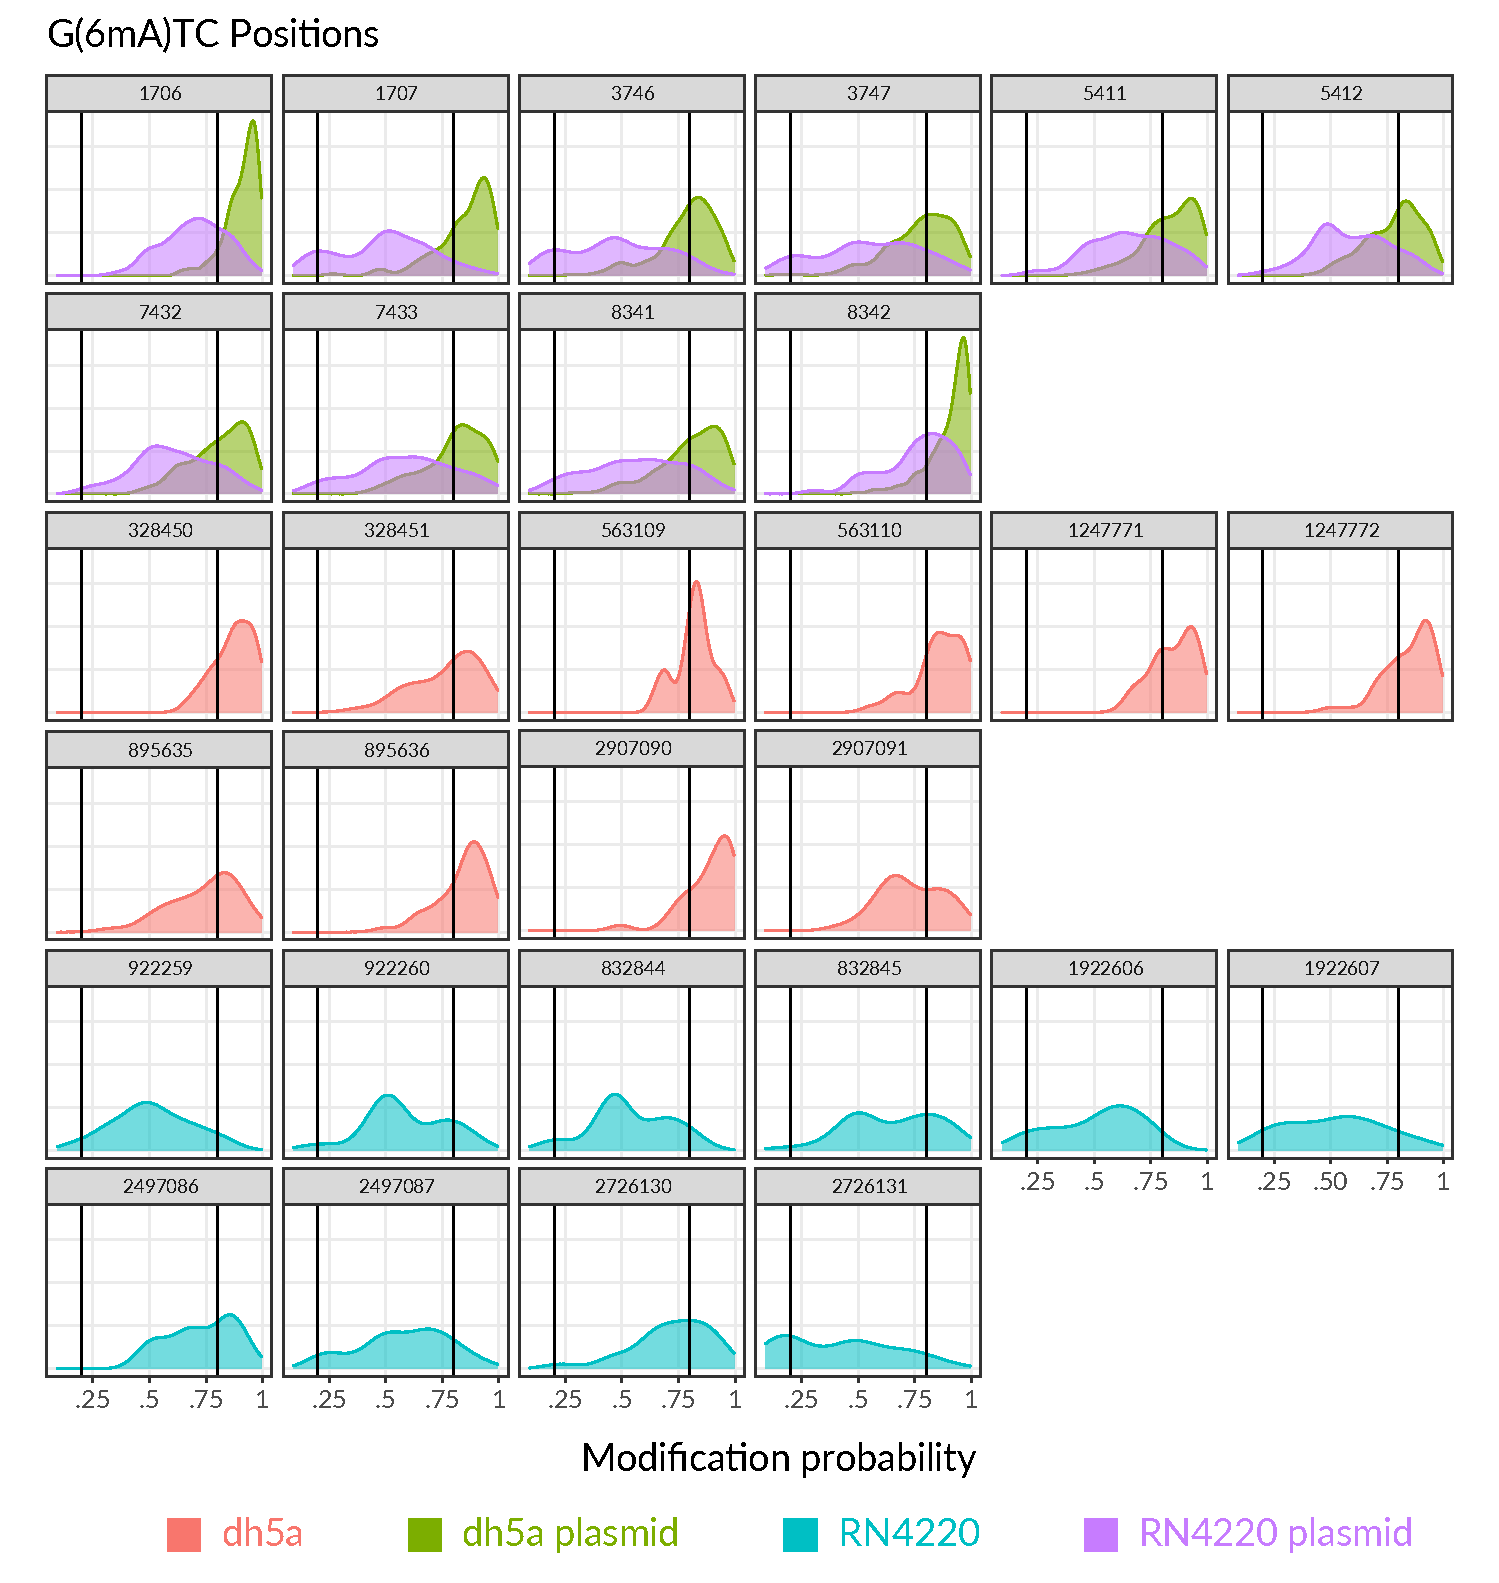
\includegraphics[width = 1\linewidth,keepaspectratio]{figure/modprobsfig.pdf}
\caption[ Methylation probability distributions at select dam methylation loci]{{\bf  Methylation probability distributions at select dam methylation loci.} Dam methylation loci, where dh5a and dh5a plasmid are methylated and RN4220 and RN4220 plasmid are not methylated. When unmethylated, the modification probability often peaks between .2 and .8, causing the majority of reads at these loci to be ignored, lowering the total number of calls for unmethylated loci (see Methods). }
\label{fig:modprobsfig}
\end{figure}



\begin{table}[!hb]
\centering
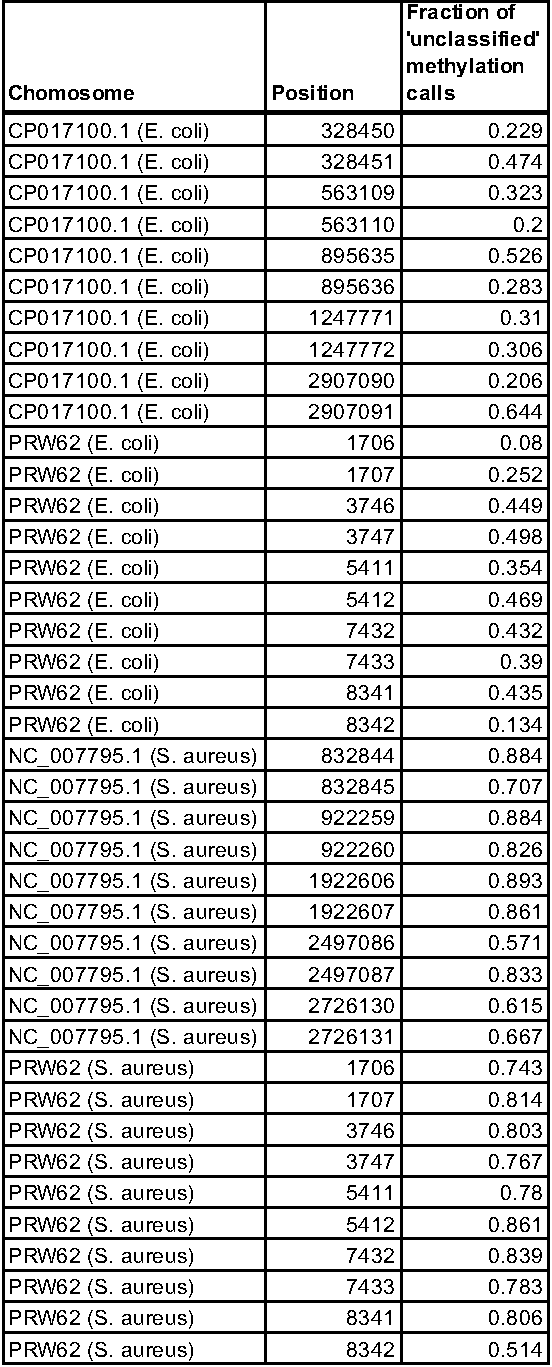
\includegraphics[width = .5\linewidth,keepaspectratio]{figure/modprobs.pdf}
\caption[Unclassified loci]{{\bf Unclassified loci.} Fraction of 'unclassified' methylation calls made at select GATC loci in S. aureus, E. coli and plasmid PRW62 in each. }
\label{tab:modprobs}
\end{table}


Ensuring an equal mixture of plasmid reads is possible in simple systems where plasmid copy numbers are known or controlled, but it is not easily applicable in complex metagenomic contexts. While unnormalized contig-level methylation signatures can be effective for correctly identifying a single host, it is less reliable for identifying multiple hosts.


\subsection{Clinical Sample}
\label{sec:mdr}

Moving away from controlled samples, we wanted to examine the performance of methylation binning on a clinical stool sample, comparing the clustering results to a matched Hi-C library to provide a “ground truth”. From Illumina shotgun sequencing data, we assembled metagenomic contigs. These contigs were then binned using a matched Hi-C library, resulting in Hi-C bins, which are collections of Illumina contigs corresponding to the genetic complement of a member of the microbial community. We also sequenced the stool metagenome using the ONT platform, assembled metagenomic contigs using the ONT reads, and then polished these contigs using ONT read alignments {\bf Table \ref{tab:asmstats}}. These polished metagenomic contigs represent segments of DNA found in the microbial community, but are not binned or otherwise grouped in any way. In order to group these contigs, we called methylation and used this methylation signal to bin the long-read contigs.


\begin{table}[!hb]
\centering
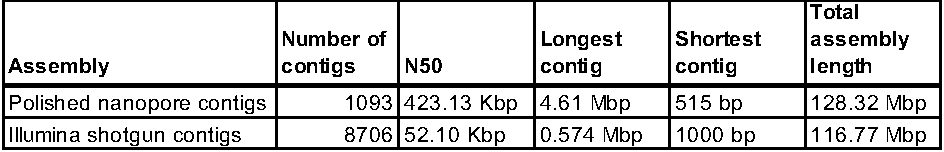
\includegraphics[width = 1\linewidth,keepaspectratio]{figure/asmstats.pdf}
\caption[Assembly summary statistics]{{\bf Assembly summary statistics.} Summary statistics for the contigs assembled with nanopore reads, and contigs assembled with Illumina reads. }
\label{tab:asmstats}
\end{table}


Because the relevant methylation motifs in this sample are unknown, we selected the most frequently occurring ones in REBASE, as recently used by \citep{Tourancheau2021-hv}, then narrowed these down further to the 14 motifs that occur at least once in each contig on a sufficient number of contigs, preferentially keeping 5mC motifs {\bf Tables \ref{tab:clinmotifs}, \ref{tab:considered}}. We calculated a methylation signature for each contig using the percent methylation at each motif, then clustered contigs using the Euclidean distance between signatures. Polished ONT contigs were then matched to Hi-C bins using whole genome alignment.

\begin{table}[!hb]
\centering
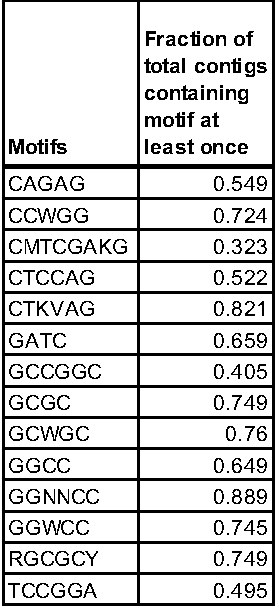
\includegraphics[width = .25\linewidth,keepaspectratio]{figure/clinmotifs.pdf}
\caption[Clinical barcode]{{\bf Clinical barcode.} Motifs used in the clinical barcode, and fraction of contigs in the clinical sample containing at least one occurence each motif used for methylation binning. }
\label{tab:clinmotifs}
\end{table}


\begin{table}[!hb]
\centering
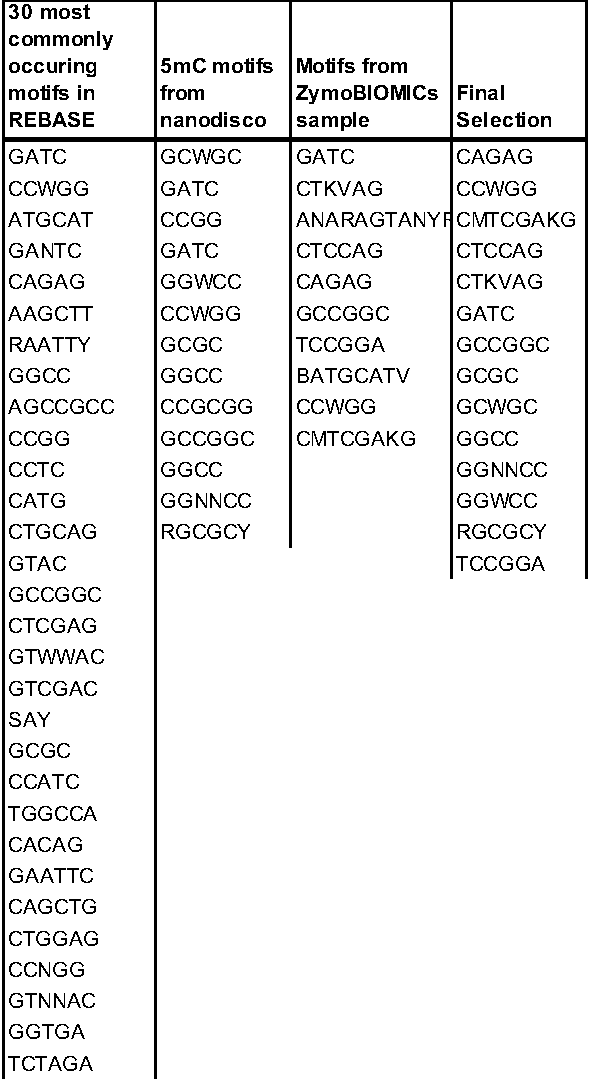
\includegraphics[width = .5\linewidth,keepaspectratio]{figure/considered.pdf}
\caption[Considered motifs]{{\bf Considered motifs.} Methylation motifs considered for the final barcode. }
\label{tab:considered}
\end{table}


To assess the performance of this methylation based clustering compared to Hi-C, we show the ‘contamination’ and ‘completeness’ of clusters as defined by different height thresholds on the tree, where height corresponds to methylation-based Euclidean distance. Here, ‘contamination’ is the percentage of contigs not contained in a cluster with only other contigs of the same Hi-C bin, while ‘completeness’ is the percentage of contigs contained in the same cluster as the majority of contigs of its bin {\bf Figure \ref{fig:mdrfig}a}. Similar to a receiver operating curve (ROC) for binary classifiers, an ideal clustering would have either 100\% 1-contamination or 100\% completeness at all height thresholds, resulting in an AUC of 1. Unlike an ROC, a random classifier would not be represented by a diagonal line, but a decay-like function, according to simulated random clustering.


\begin{figure}[!hb]
\centering
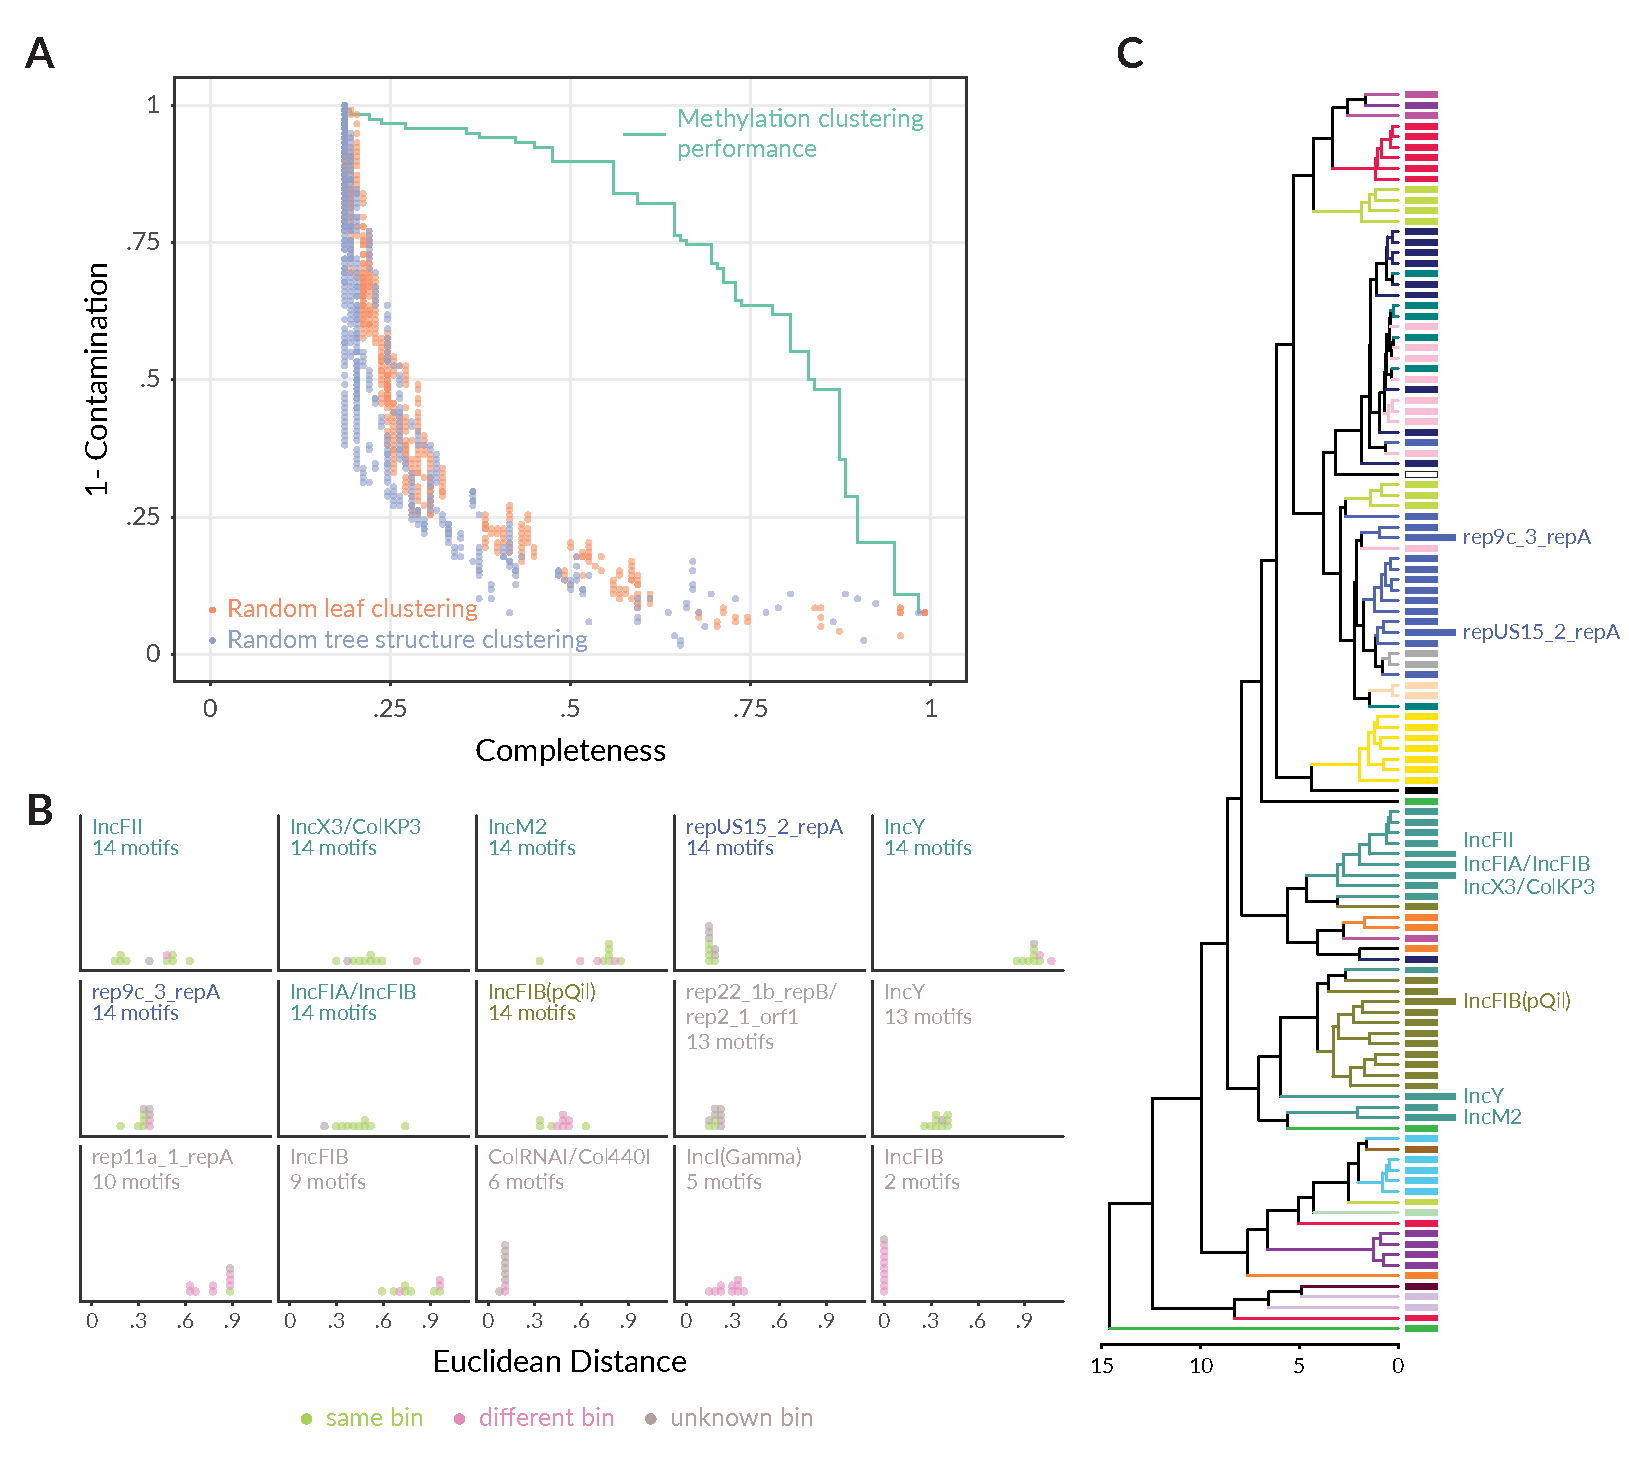
\includegraphics[width = 1\linewidth,keepaspectratio]{figure/mdrfig.pdf}
\caption[Methylation binning of a clinical sample compared to Hi-C]{{\bf Methylation binning of a clinical sample compared to Hi-C.} {\bf (A)} 1-Contamination vs. Completeness curve of methylation-based hierarchical clustering of clinical metagenomic contigs. Simulations of random clustering performance are shown using points. {\bf (B)} Tree showing hierarchical clustering of contigs, where colors represent Hi-C bins assigned to each contig. Contigs representing plasmids are shown with labels. {\bf (C)} Distance distributions between each plasmid contig and the 20 closest contigs to each by methylation distance. Contigs are colored by whether they belong to the same Hi-C bin as the plasmid contig. }
\label{fig:mdrfig}
\end{figure}



Moving to mobile elements, we found that contigs identified as plasmids belong to the same methylation distance clusters as Hi-C bins.  For all eight plasmid contigs with full barcode information,  the nearest contigs come from the same bin {\bf Figure \ref{fig:mdrfig}b,c}. While these pairwise distance calculations can be done using a subset of motifs in the barcode if a plasmid contig does not contain all the motifs, the number of nearby contigs belonging to the same bin decreases as motifs are removed {\bf Figure \ref{fig:mdrfig}c}.

Using PlasmidFinder, we identified which nanopore contigs were likely to be plasmids, and using Kraken2, we classified them taxonomically. Of the nanopore contigs identified as plasmids, three were classified as K. pneumoniae sequences. These were an IncFIB(pQil) plasmid, an IncM2 plasmid, and a plasmid identified as both IncX3 and ColKP3. However, the IncM2 and the IncX3/ColKP3 plasmids align to a Hi-C bin that is predominantly composed of E. coli sequences (bin\_3), suggesting that E. coli was the host organism for these plasmids in the original sample. Methylation distance corroborates this, as the nearest contigs to these two plasmid contigs are also both classified as E. coli sequences. However, a ColKP3 sequence was detected in the Illumina contigs making up the K. pneumoniae Hi-C bin\_5. While this could indicate a mis-assembly of the IncX3/ColKP3 nanopore contig, coverage profiles across each plasmid contig did not exhibit any stepwise or aberrant changes. Furthermore, the flye assembler indicates that the IncX3/ColKP3 contig is circular, suggesting that mis-assembly is unlikely, though not impossible. Without using orthogonal information from either Hi-C or methylation, correctly identifying the host of these plasmids as E. coli would not have been possible.

\section{Discussion}
\label{sec:discuss}

With the drop in sequencing costs and the development of new computational tools, metagenomic sequencing has risen to be an incredibly useful tool to profile microbial samples for ecology and health research. However, problems still arise with appropriate identification of MGEs, i.e. phages, plasmids, insertion elements - where the sequence could theoretically belong to any of the hosts present in the sample. Though there are ways to profile these currently - either through culture-based proximity ligation methods, they are costly in time and treasure. Instead, using the methylation signals embedded in nanopore sequencing data can be directly useful for metagenomic binning applications. Here we have outlined a method to do so from a typical sequencing run, without the need for any additional paired sequencing runs or data acquisition. While this work represents a starting point for these binning applications, it is currently limited in several key ways.

Currently, non-5mCG methylation calling on the ONT platform does not consistently yield calls of the same confidence or quality as CG methylation calls. Because of this, the methylation status at many of these low confidence loci are left undetermined. We have shown that aggregation of methylation calls, both across reads and along contigs, can mitigate this issue, so that contig bin and plasmid assignments can be accurately made. This is aided by the long contigs generated from long-read metagenome assembly - longer contigs have a better chance of containing a given methylation motif. However, as methylation calling continues to improve on long-read sequencing platforms discriminatory power will also improve.

Additionally, the lack of specific methylation information presents a challenge, as constructing methylation signatures requires some prior knowledge of the motifs likely to give high differentiating power. With a highly comprehensive bacterial methylation database, motifs can be chosen based on the species and strain composition of the sample as elucidated by sequence information. While REBASE is an excellent resource to start with \citep{Roberts2003-ss}, it lacks some 5mC motifs of common bacterial strains \citep{Tourancheau2021-hv}. For example, the TC(5mC)GGA motif identified in the E. coli strain (Castellani and Chalmers 1919) of the Zymo community was not listed with any E. coli strain in REBASE, and the CMT(5mC)GAKG motif found in the Zymo P. aeruginosa (PRD-10) was not listed at all in the database. However, recent work on motif discovery has been promising \citep{Tourancheau2021-hv, Beaulaurier2018-mu}, and will continue to improve knowledge of bacterial methylomes in combination with more widespread bacterial bisulfite sequencing \citep{Oliveira_Pedro_H2021-rs}. These insights will better inform motif selection and significantly improve binning efforts, as well as further the field of bacterial epigenetics generally.

Lastly, the applicability of this method is limited because of its inability to identify plasmids in multiple hosts. However, it does not escape our notice that given the long-read nature of nanopore sequencing, it may be possible to aggregate methylation signals along whole reads, and classify them as has been done with PacBio data \citep{Beaulaurier2018-mu}. Again, this will become more feasible as methylation calling on the platform continues to improve.

Despite these current limitations, we find that it is possible to bin some single-host plasmids on a single ONT sequencing run, which can be a useful supplement to kmer-based and coverage-based binning software. As sequencing power becomes more democratized and microbial surveillance needs become more urgent \citep{Iskandar2021-eg}, further development of similar low-barrier metagenomic methods will be necessary.


\section{Methods}
\label{sec:methods}

\subsection{Strain culture}
\label{sec:methods}

Staphylococcus aureus RN4220 cells were grown at 37°C in Bacto Brain-Heart infusion (BHI) broth with shaking at 220 RPM. Antibiotics were used at the following concentrations for strain construction and plasmid maintenance in S. aureus: spectinomycin, 250 µg/mL. Escherichia coli Dh5a cells were grown at 37°C, unless otherwise indicated, in RPI Luria Broth (LB) with spectinomycin at 50 µg/mL for plasmid maintenance. Strains were constructed, stored in 10\% DMSO in -80°C, and restruck on BHI agar (S. aureus) or LB agar (E. coli) with spectinomycin if needed.

pRW62 was constructed by Gibson assembly using the pLZ12 backbone (primers JW713/714) and from a construct (pDB184) containing the Streptococcus pyogenes CRISPR-Cas locus from strain SF370 (JW715/754) with a single spacer. Plasmids were transformed into chemically competent Dh5a with heat shock or electrocompetent RN4220 with electroporation, then plated on antibiotic for selection.e.

\subsection{DNA extraction and sequencing}
\label{sec:methods}

The ZymoBIOMICS HMW DNA Standard was purchased from Zymo Research. From this, an ONT sequencing library was prepared using the ONT ligation based sequencing kit (SQK-LSK109) according to manufacturer specifications {\bf Table \ref{tab:yields}}.

DNA was extracted from strains 3294 and 3689 (see Strain culture above) using the Zymo Quick-DNA Fungal Bacterial Kit, and sequenced using the ONT Rapid Sequencing Kit (SQK-RAD004) and a flongle flowcell (FLO-FLG001). For bisulfite sequencing, DNA was sheared to 300bp using the Bioruptor Pico according to manufacturer specifications. Bisulfite conversion was done using the Zymo EZ DNA Methylation Gold Kit, and a sequencing library was prepared using the Swift Accel-NGS Methyl-Seq DNA Library Kit, all according to manufacturer specifications.

DNA was extracted from a human stool sample collected at the Johns Hopkins Hospital Medical Microbiology Laboratory using the Qiagen PowerSoil DNA Isolation Kit, and an ONT library was prepared again using the ligation based sequencing kit (SQK-LSK109). These libraries were then sequenced on a FLO-MIN106D (R9.4.1) flowcell using a GridION. From the same stool sample, a proximity ligation (Hi-C) library was prepared using the Phase Genomics ProxiMeta Kit. The accompanying shotgun library was prepared also using the Qiagen PowerSoil DNA Isolation Kit for extraction, and the Illumina Nextera DNA Flex Library Prep Kit. Both the Hi-C library and the shotgun library were sequenced on a HiSeq 2500 using 2x100 chemistry.


\subsection{Assembly and alignment}
\label{sec:methods}

All ONT data was bascalled using the Guppy basecaller (v4.5.2) with the high accuracy model appropriate to the R9.4.1 flowcells used (dna\_r9.4.1\_450bps\_hac). Reads with a quality score less than 9 were discarded and not used for further analysis. Any reads from the clinical stool sample aligning to the GRCh38 human reference genome using minimap2 (v2.17-r974-dirty) \citep{Li2018-eq}  with the ONT data preset map-ont were also discarded and not used for further analysis. These reads were then assembled using Flye (v2.9-b1768) \citep{Kolmogorov2020-rm}, with the –-meta flag, with the genome size set to 100Mb. Using minimap2 \citep{Li2018-eq} reads were aligned back to the assembly using the ONT data preset map-ont. The assembly was then polished with the aligned reads using racon \citep{Vaser2017-zk}(v1.4.19) with settings -m 8 -x -6 -g -8 -w 500. To further correct the assembly, Medaka (v1.4.3) was used on default settings with the r941\_min\_high\_g360 model.

\subsection{Hi-C binning and contig identification}
\label{sec:methods}

Human reads were removed from the Hi-C data using BMTagger (v3.101) \citep{Rotmistrovsky2011-ak}. Hi-C bins were calculated using the Phase Genomics platform ProxiWrap. Metagenomic contigs were assigned to Hi-C bins based on whole genome alignments made using Mummer (v4.0.0) \citep{Marcais2018-mm}. For each contig, the total contig coverage by each bin was calculated, and the bin with the highest coverage was assigned to the contig. Contigs with less than 20\% coverage by any bin were not assigned and excluded from bin analysis. Nanopore contigs were classified taxonomically using Kraken (v2.1.2) using the ‘standard’ database \citep{Wood2019-uy}.

\subsection{Methylation calling}
\label{sec:methods}

Methylation was called from nanopore data with the ONT package Megalodon (v2.3.1, https://github.com/nanoporetech/megalodon), using an all-context 5mC and 6mA model (res\_dna\_r941\_min\_modbases-all-context\_v001) available in Rerio (https://github.com/nanoporetech/rerio). For strains 3294 and 3689, the previously published E. coli NEB 5-alpha genome (accession: CP017100.1) and the S. aureus representative genome (accession: NC\_007795.1) were used as the reference genomes for anchoring methylation calls. Genomes of the organisms included in the documentation were used as the references for the ZymoBIOMICS HMW DNA Standard. The polished metagenomic assembly (see Assembly above) was used as the reference for the clinical stool sample.

For each read, bases with >80\% methylation probability were identified as methylated, while bases with <20\% methylation probability were identified as unmethylated, as per the default settings of the tool. The percent methylation at each genomic locus was determined by dividing the number of reads methylated at that locus by the total number of reads called at that locus. Reads with indeterminate methylation calls at the locus were not considered in this calculation.

\subsection{Alignment and coverage}
\label{sec:methods}

ONT reads were aligned to their respective reference genomes using minimap2 with preset map-ont. Coverage was calculated using the coverage module in bedtools (v2.27.1) \citep{Quinlan2010-lu}.

\subsection{Bisulfite analysis}
\label{sec:methods}

Whole genome bisulfite sequencing (WGBS) data for each of the 7 strains included in the Zymo community standard was obtained from SRA (BioProject PRJNA477598). Bismark (v0.23.0) \citep{Krueger2011-cu} was used to align the WGBS data for each strain to the ZymoBIOMICS reference genomes (see Methylation calling above). Genomic loci with >90\% methylation frequency were considered methylated.Methylated loci exactly matching GAT5mC or C5mCWGG were counted and tabulated {\bf Table \ref{tab:bisulf}}. Methylated loci not matching GAT5mC or C5mCWGG were visually inspected, and an overrepresentation of TC5mCGGA and GC5mCGGC methylation context was observed in E. coli, while an overrepresentation of CMT(5mC)GAKG was observed in P. aeruginosa. These contexts were then also counted and tabulated. The remaining methylated loci were then counted and tabulated as ‘unknown’ methylation contexts.

Likewise in the bisulfite data of the two-bacteria system, Bismark was used to align the WGBS reads to the reference genomes, and only genomic loci with >90\% methylation frequency were considered methylated. All methylated loci on the E. coli genome were determined to exactly match the C5mCWGG context. The two methylated loci found on the S. aureus genome did not match C5mCWGG and were not further contextualized.

\subsection{Data Availability}
\label{sec:methods}

All data is available in the European Nucleotide Archive (ENA) Study Accession PRJEB54092. All code used for analysis is freely available for download at https://github.com/timplab/fan\_methbin.
